\documentclass[10pt,twocolumn]{article}
\usepackage[margin=0.75in]{geometry}                % See geometry.pdf to learn the layout options. There are lots.
\geometry{letterpaper}                   % ... or a4paper or a5paper or ... 
%\geometry{landscape}                % Activate for for rotated page geometry
%\usepackage[parfill]{parskip}    % Activate to begin paragraphs with an empty line rather than an indent
\setlength{\columnsep}{1cm}
\usepackage{graphicx}
\usepackage{amssymb}
\usepackage{epstopdf}
\usepackage{fullpage}
\usepackage[usenames]{color}
\usepackage{titlesec}
\usepackage{hyperref}
\usepackage{framed}
\usepackage{algorithmic}

\definecolor{light-gray}{gray}{0.45}
\titleformat{\section}
{\color{black}\normalfont\Large\bfseries}
{\color{black}\thesection}{1em}{}

\titleformat{\subsection}
{\color{light-gray}\normalfont\large\bfseries}
{\color{light-gray}\thesubsection}{1em}{}

\DeclareGraphicsRule{.tif}{png}{.png}{`convert #1 `dirname #1`/`basename #1 .tif`.png}

\title{\Huge{\bf Algorithm 5: Ray}}
\author{Comp175: Introduction to Computer Graphics -- Spring 2016}
\date{Algorithm due:  {\bf Monday April 11th} at 11:59pm}                                         % Activate to display a given date or no date

\begin{document}
\maketitle
%\section{}
%\subsection{}

\begin{verbatim}
Your Names: ____Matt_Asnes________________

            ____Adam_Plumer_______________

Your CS Logins: ____masnes01______________

                ____ap____________________
\end{verbatim}

\section{Instructions}
Complete this assignment only with your teammate. When a numerical answer is required, provide a reduced fraction (i.e. 1/3) or at least three decimal places (i.e. 0.333). Show all work; write your answers on this sheet. This algorithm handout is worth 3\% of your final grade for the class.

\begin{framed}
\noindent{\bf[2 points]} The high-level view of our ray tracer is exactly the same as for intersect, except for a few additions. Below is the high-level pseudocode for {\tt Intersect}. What needs to be changed/added to make this a full-fledged raytracer? Just specify what changes need to be made {no pseudocode please.}

\footnotesize{
\begin{algorithmic}
\FOR{$point \in Canvas$}
	\STATE Cast a ray to find the nearest object
	\IF{ray intersects an object}
		\FOR{each light}
			\STATE Cast a ray to the light and evaluate the lighting equation\\
			\STATE $Canvas[pt] = Canvas[pt]+ color$ with only diffuse/ambient components\\
		\ENDFOR
	\ELSE 
		\STATE $Canvas[pt] =$ background color
	\ENDIF
\ENDFOR
\end{algorithmic}
}

We need to add specular lighting, add directional lights, make the raytracer recursive to support shadows and reflections, and add texture mapping for simple solids. This will mostly involve changes to the lighting equation (specular light is an additive term, directional lights change $L_i$, the recursive component is additive and may require some changes to our lighting function, and texture mapping requires changes to how we handle object normals).
\end{framed}

\begin{framed}
\noindent{\bf[2 points]} Given a vector $\vec{v}$ and a surface normal $\vec{n}$, find the equation for the vector $\vec{r}$ which is the reflection of $\vec{v}$ about $\vec{n}$ (i.e. in the equal and opposite direction). Write your equation in terms of vector operations. How do you compute the color contributed by the reflected ray? Give a brief description.
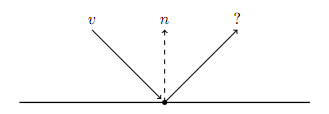
\includegraphics[width=2.8in]{reflection.png}

Call the reflected ray $r$, and denote the vector from the endpoint of $n$ to the origin of $v$ as $a$ (this will cancel out). Then:

\[r = n (-v \cdot n) + a\]
As the dot product will project $-v$ onto $n$, and adding $a$ will bring us over to where $r$ is. Similarly:
\[-v + a = n (v \cdot n)\]
Then:
\[r = 2 n (-v \cdot n) + v = v - 2 n (r \cdot n) \]

\end{framed}

\begin{framed}
\noindent{\bf[1 point]} Is ray tracing a local or global illumination algorithm? Why?

Global, since although it is computed via direct illumination of a surface from a light source, the recursive components take into account the global state of the world and all objects in it. If we computed based only on an ambient light term and the eye and light positions, we would have a local model of direct illumination; however as soon as other objects directly impact the drawing of another object, the lighting model becomes global.
\end{framed}

\begin{framed}
\noindent{\bf[1 point]} For a particular ray that intersects with an object, when do you not consider contribution from a given light source? How do you computationally determine when this scenario occurs?

When the light is behind the object (as direct light from it will not impact the color) we do not want to compute direct contributions from that light source (though we \textit{do} still want to compute recursive terms). This scenario occurs when the dot product of the normal and the incident light ray is negative.
\end{framed}

\begin{framed}
\noindent{\bf[2 points]} Recall that we can think of texture mapping in two steps. First, mapping from the object to the unit square, and second, mapping from the unit square to the texture map. Let $u$ and $v$ be the $x$ and $y$ values in the unit square that a particular point on an object gets mapped to in the first step. Note that $a$ and $b$ are calculated differently depending on the object. From here, how do you find the coordinates $(s, t)$ to look up in a texture map in terms of $u, v, i, j, w$ and $h$, where $i$ and $j$ are the number of repetitions in the $x$ and $y$
directions, respectively, $w$ is the texture width, and $h$ is the texture height?
\vskip 12em
\end{framed}
\vskip 6em

\begin{framed}
\noindent{\bf[1 point]} How do you use the color from the texture map and the {\tt blend} value in the lighting equation?
\vskip 12em
\end{framed}

\begin{framed}
\noindent{\bf[1 point]}  What is the Phong lighting model used for? What is the purpose of its exponent?\\

The Phong model is used for real-time rendering because it is a local illumination model; its exponent is used to determine the shininess of the material in terms of specular light.
\end{framed}

\section{How to Submit}

Hand in a PDF version of your solutions using the following command:
\begin{center}
 {\tt provide comp175 a5-alg}
 \end{center}
\end{document}  
